\documentclass{beamer}

%%% Usepackage
% Basic
\usepackage{amsmath}   % Math input support
\usepackage{amssymb}   % Math input support
\usepackage{booktabs}  % 3 line table show
\usepackage{float}     % Figure and Table env.
\usepackage{makecell}  % Mult. lines in one table cell
\usepackage{bm}

% Color Support
\usepackage{xcolor}
\definecolor{commcolor}{rgb}{0,0.6,0}
\definecolor{rulesepcolor}{rgb}{0.2,0.2,0.2}
\definecolor{stringcolor}{rgb}{0.58,0,0.82}
\definecolor{backcolor}{rgb}{0.93,0.87,0.89}
\definecolor{backcolor2}{rgb}{1,1,0.9}
\definecolor{pergray}{rgb}{0.88,0.88,0.88}

% Coding block
\usepackage{listings}
\lstset{
  language=python,
  basicstyle=\tiny\ttfamily,
  captionpos=b,
  backgroundcolor=\color{backcolor2},
  commentstyle=\color{commcolor},
  escapeinside={\%*}{*)},
  keywordstyle=\color{blue},
  stringstyle=\color{stringcolor}\ttfamily,
  frame=none,
  rulesepcolor=\color{rulesepcolor},
  numbers=left,
  numbersep=4pt,
  numberstyle={\color[RGB]{170,170,170}},
  % xleftmargin=1.5em,
  % xrightmargin=1.5em,
}

% Coding block smooth
\usepackage{tikz}
\usepackage[framemethod=tikz,skipbelow=\topskip,skipabove=\topskip]{mdframed}
\mdfsetup{
  leftmargin=0pt,
  rightmargin=0pt,
  backgroundcolor=backcolor2,
  middlelinecolor=backcolor2,
  roundcorner=5pt,
}
\usepackage{etoolbox}
\BeforeBeginEnvironment{lstlisting}{\begin{mdframed}\vspace{-1em}}
\AfterEndEnvironment{lstlisting}{\vspace{-1em}\end{mdframed}}

% Inline coding
\usepackage{newverbs}
\newverbcommand{\cverb}
  {\setbox\verbbox\hbox\bgroup}
  {\egroup\tcbox{\color{purple}\box\verbbox}}

% Picture shadow box & Inline coding bg
\usepackage[many]{tcolorbox}
\tcbset{
  on line,
  boxsep=0.6pt, 
  left=0pt, right=0pt, top=0pt, bottom=0pt,
  colframe=backcolor, 
  colback=pergray,  
  highlight math style={enhanced}
}


%%% New command
\newcommand{\purple}{\textcolor{purple}}


%%% Page style
\setbeamertemplate{navigation symbols}{}
\usefonttheme{professionalfonts}
\usetheme{Madrid}
\usecolortheme{default}


%%% Pages
%+===================================================================+%
\title{The 2nd station to DMFT: DFT+U}
\subtitle{(After you know what is Anderson impurity model.)}

\author[Yang Li]{
  Yang Li\inst{1}}  
\institute[CMT Tsinghua Univ.]{
  \inst{1} Department of Physics\\Tsinghua University 
}

\date[Nov. 2022]{Nov. 2022}
%-===================================================================-%

\begin{document}
  %+===================================================================+%
  \frame{\titlepage}
  %-===================================================================-%

  %+===================================================================+%
  \begin{frame}{When does the DFT not work?}
    \begin{block}{Answer in short}
      The traditional density functional theory (DFT) calculation method is not working when processing strongly correlated materials, like Mott insulators.
    \end{block}

    \begin{block}{Answer in bullshit}
      DFT is not working when it is not working.
    \end{block}

    \begin{block}{Answer ask more questions}
      You must first know why the DFT is not working. Then we can determine when it will fail.
    \end{block}
    
  \end{frame}
  %-===================================================================-% 

  %+===================================================================+%
  \begin{frame}{Why does the DFT not work?}
    Hartree-Fock (HF) approximation (without spin),
    \begin{equation}\scriptsize
      \begin{aligned}
        E^{\text{HF}}_j\phi_j(\bm{r}) &= \left[-\frac{\hbar^2}{2m}\nabla^2+V(\bm{r})\right]\phi_j(\bm{r}) \\
        &+ \frac{e^2}{4\pi{}\varepsilon_0}\sum_k\int\frac{\phi_k^*(\bm{r'})\phi_k(\bm{r'})}{|\bm{r}-\bm{r'}|}\mathrm{d}^3r'\; \phi_j(\bm{r}) \\
        &- \frac{e^2}{4\pi{}\varepsilon_0}\sum_k\int\frac{\phi_j^*(\bm{r'})\phi_k(\bm{r'})}{|\bm{r}-\bm{r'}|}\mathrm{d}^3r'\; \phi_k(\bm{r})
      \end{aligned}
    \end{equation}
    \begin{block}{Delocalization error (\emph{i.e.}, many-body self-interaction error)}
      The LDA or GGA, which only uses the electron density's information, is insufficient for precisely describing the exchange effect. It will introduce some residual self-interaction energy, which will make the Coulomb interaction overestimate and the electrons tend to be more delocalized, \purple{especially in \(d\)/\(f\) orbits.}
    \end{block}
  \end{frame}
  %-===================================================================-% 

  %+===================================================================+%
  \begin{frame}{Why does the DFT not work?}
    HF approximation (without spin),
    \begin{equation*}\scriptsize
      \begin{aligned}
        E^{\text{HF}}_j\phi_j(\bm{r}) &= \left[-\frac{\hbar^2}{2m}\nabla^2+V(\bm{r})\right]\phi_j(\bm{r}) \\
        &+ \frac{e^2}{4\pi{}\varepsilon_0}\sum_k\int\frac{\phi_k^*(\bm{r'})\phi_k(\bm{r'})}{|\bm{r}-\bm{r'}|}\mathrm{d}^3r'\; \phi_j(\bm{r}) \\
        &- \frac{e^2}{4\pi{}\varepsilon_0}\sum_k\int\frac{\phi_j^*(\bm{r'})\phi_k(\bm{r'})}{|\bm{r}-\bm{r'}|}\mathrm{d}^3r'\; \phi_k(\bm{r})
      \end{aligned}
    \end{equation*}

    \begin{block}{Static correlation error (HF method also has this problem)}
      DFT is based on the single-electron approximation and puts the complex many-body correlation into the exchange correlation term. Both LDA and GGA functionals are fitted from the numerical results of the homogeneous electron gas model, which only depend on the local density and the gradient of the local density, ignoring the time and space fluctuations of complex many-body correlations. \purple{The dynamic correlation effect of strongly correlated \(d\)/\(f\) electrons cannot be described.}
    \end{block}
  \end{frame}
  %-===================================================================-% 

  %+===================================================================+%
  \begin{frame}{What can we do when DFT fails?}
    Many approaches have been proposed to address these deficiencies, such as,
    \begin{itemize}
      \item self-interaction corrected DFT, \href{https://doi.org/10.1103/physrevb.23.5048}{\textcolor{blue}{\tiny[Phys. Rev. B 23, 5048 (1981)]}}
      \item hybrid functionals, \href{https://doi.org/10.1063/1.464913}{\textcolor{blue}{\tiny[J. Chem. Phys. 98, 5648 (1993)]}}
      \item the localized orbital scaling correction, \href{https://doi.org/10.1093/nsr/nwx111}{\textcolor{blue}{\tiny[Natl. Sci. Rev. 5, 203 (2018)]}}
      \item fractional spin correction. \href{https://doi.org/10.1073/pnas.1807095115}{\textcolor{blue}{\tiny[Proc. Natl. Acad. Sci. U. S. A. 115, 9678 (2018)]}}
      \item ...
    \end{itemize}

    \begin{block}{The most popular method}
      The most popular approaches in solid-state physics are the combination of L(S)DA and GGAs
      \begin{itemize}
        \item with a simpler mean-field-type correction based on the Hubbard model (DFT+\(U\)), \href{https://doi.org/10.1103/physrevb.44.943}{\textcolor{blue}{\tiny[Phys. Rev. B 44, 943 (1991)]}}
        \item and with the non-perturbative manybody technique-dynamical mean-field theory (DMFT). \href{https://doi.org/10.1103/PhysRevLett.62.324}{\textcolor{blue}{\tiny[Phys. Rev. Lett. 62, 324 (1989)]}}
      \end{itemize}
    \end{block}

  \end{frame}
  %-===================================================================-% 

  %+===================================================================+%
  \begin{frame}{The basic idea of DFT+\(U\) method}
    \begin{equation}
      E_{\text{DFT+}U} = E_{\text{DFT}} - E_{\text{dc}} + E_{U}
    \end{equation}

    \begin{block}{Pickup artist}
      \begin{itemize}
        \item \(E_{\text{DFT}}\) is the energy of density functional approximations at the level of L(S)DA or GGA.
        \item \(E_{U}\) is the Coulomb interaction energy due to strongly correlated electrons given by the \purple{Hartree-Fock approximation to the multi-orbital Hubbard model}.
        \item The double counting term \(E_{\text{dc}}\) is subtracted here to discount the Coulomb interaction energy that is already included in DFT at an average level.
      \end{itemize}
    \end{block}
  \end{frame}
  %-===================================================================-% 

  %+===================================================================+%
  \begin{frame}{The \(E_U\) term: multi-orbital Hubbard model}
    The full electron-electron interaction can be written as,
    \begin{equation}
      \hat{H}_{\text{Hub}} = \frac{1}{2}\sum_{\{m\}}\sum_{\sigma{}\sigma'}\langle{}mm'|v_{\text{sc}}|m''m'''\rangle\hat{c}_{m}^{\sigma{}\dagger}\hat{c}_{m'}^{\sigma'{}\dagger}\hat{c}_{m'''}^{\sigma'}\hat{c}_{m''}^{\sigma}
    \end{equation}

    Where the Coulomb interaction matrix elements are,
    \begin{equation}
      \langle{}mm'|v_{\text{sc}}|m''m'''\rangle = \int\;\mathrm{d}\bm{r}\mathrm{d}\bm{r'}\; \phi_m^*(\bm{r})\phi_{m'}^*(\bm{r'})v_{\text{sc}}(\bm{r}, \bm{r'})\phi_{m''}(\bm{r})\phi_{m'''}(\bm{r'})
    \end{equation}
    
    And \(v_{\text{sc}}\) is the statically screened Coulomb potential, \(\{m\}\) represent \(m,m',m'',m'''\) are the local orbital indices for \(d\) or \(f\) subshell.
  \end{frame}
  %-===================================================================-% 

  %+===================================================================+%
  \begin{frame}{The \(E_U\) term: Hartree-Fock approximation}
    Neglecting the spin-orbit coupling (SOC) effect, the \purple{Hartree-Fock approximation} to the Hubbard Hamiltonian can be obtained by evaluting its expectation value within the symmetrical Kohn-Sham (KS) ground state \(|0\rangle\).

    \begin{equation}\label{eq:EU}
      \begin{aligned}
        E_U &= \langle{}0|\hat{H}_{\text{Hub}}|0\rangle\\
            &= \frac{1}{2}\sum_{\{m\},\sigma}\left(\langle{}mm'|v_{\text{sc}}|m''m'''\rangle - \langle{}mm'|v_{\text{sc}}|m'''m''\rangle\right)n_{m''m}^{\sigma}n_{m'''m'}^{\sigma}\\
            &+ \frac{1}{2}\sum_{\{m\},\sigma}\langle{}mm'|v_{\text{sc}}|m''m'''\rangle{}n_{m''m}^{\sigma}n_{m'''m'}^{-\sigma}
      \end{aligned}
    \end{equation}
    Where the \(n_{mm'}^{\sigma}\) is the local occupation matrix given by,
    \begin{equation}
      n_{mm'}^{\sigma} = \langle{}0|\hat{c}^{\sigma\dagger}_{m'}\hat{c}^{\sigma}_{m}|0\rangle = \frac{1}{N_{\bm{k}}}\sum_{n,\bm{k}}f^\sigma_{n\bm{k}}\langle\psi^\sigma_{n\bm{k}}|m'\sigma\rangle\langle{}m\sigma|\psi^\sigma_{n\bm{k}}\rangle
    \end{equation}
  \end{frame}
  %-===================================================================-% 

  %+===================================================================+%
  \begin{frame}{The \(E_U\) term: rotationally invariant and diagonalize}
    \begin{block}{Observations}
      \begin{itemize}
        \item Since the \(E_U\) is a observable quantity, Eq. \eqref{eq:EU} must be rotationally invariable.
        \item The occupation number matrix \(n^{\sigma}\) is hermitian, one can always introduce a unitary transformation to diagonalize it.
      \end{itemize}
    \end{block}
    \begin{equation}\label{eq:EU2}
      E_U = \frac{1}{2}U\sum_{mm',\sigma}\bm{n}^\sigma_{m}\bm{n}^{-\sigma}_{\bm{m'}} - \frac{1}{2}(U-J)\sum_{m\ne{}m',\sigma}\bm{n}^\sigma_{m}\bm{n}^{\sigma}_{\bm{m'}}
    \end{equation}
    \begin{subequations}
      \begin{align}
        U &= \langle{}mm'|v_{\text{sc}}|mm'\rangle\\
        J &= \langle{}mm'|v_{\text{sc}}|m'm\rangle
      \end{align}
    \end{subequations}
    Note that the self-interaction is absent in both Eq. \eqref{eq:EU} and Eq. \eqref{eq:EU2}.
  \end{frame}
  %-===================================================================-% 

  %+===================================================================+%
  \begin{frame}{The \(E_\text{dc}\) term: fully localized limit (FLL) scheme}
    The double counting term \(E_\text{dc}\)is an important portion of the DFT+\(U\) theory. But the local/semi-local DFT are not orbit-resolved theories. Contributions from individual orbitals cannot be well separatd.

    \begin{block}{Double counting schemes}
      By now, there are two main \(E_\text{dc}\) schemes used in DFT+\(U\) calculation. 
      \begin{itemize}
        \item One is called ``around mean field (AMF)'' scheme, which gives a better description for metallic system. \href{https://doi.org/10.1103/physrevb.44.943}{\textcolor{blue}{\tiny[Phys. Rev. B 44, 943 (1991)]}}
        \item The other is called ``fully localized limit (FLL)'' scheme, which is more suitable for insulating system. \href{https://doi.org/10.1103/PhysRevB.79.035103}{\textcolor{blue}{\tiny[Phys. Rev. B 79, 035103 (2009)]}}
      \end{itemize}
    \end{block}
    \begin{equation}
      E_\text{dc}^{\text{FLL}} = \frac{1}{2}UN(N-1) - \frac{1}{2}J\sum_\sigma{}N^\sigma(N^\sigma{}-1).
    \end{equation}
  \end{frame}
  %-===================================================================-% 

  %+===================================================================+%
  \begin{frame}{The final expression for DFT+\(U\) method}
    \begin{equation*}\textcolor{gray}{\small\begin{aligned}
      E_{\text{DFT+}U} &= E_{\text{DFT}} - E_{\text{dc}} + E_{U}\\
      E_U &= \frac{1}{2}U\sum_{mm',\sigma}\bm{n}^\sigma_{m}\bm{n}^{-\sigma}_{\bm{m'}} - \frac{1}{2}(U-J)\sum_{m\ne{}m',\sigma}\bm{n}^\sigma_{m}\bm{n}^{\sigma}_{\bm{m'}}\\
      E_\text{dc} &= \frac{1}{2}UN(N-1) - \frac{1}{2}J\sum_\sigma{}N^\sigma(N^\sigma{}-1).
    \end{aligned}}\end{equation*}

    Note that, \(N = \sum_{\sigma} N^\sigma = \sum_{m,\sigma}\bm{n}^{\sigma}_{m}\). Then,
    \begin{equation}
      \begin{aligned}
        \Delta{}E_{\text{DFT+}U} &= E_{\text{DFT+}U} - E_{\text{DFT}}\\
        &= \frac{1}{2}(U-J)\sum_{m,\sigma}(\bm{n}^{\sigma}_{m} - \bm{n}^{\sigma}_{m}\bm{n}^{\sigma}_{m})
      \end{aligned}
    \end{equation}

    \begin{block}{Wait, are they?}
      If the parameters \(U\) and \(J\) are exact, then the self-interaction will be greatly eliminated.
    \end{block}
  \end{frame}
  %-===================================================================-% 

  %+===================================================================+%
  \begin{frame}{What about the value of \(U\) and \(J\)?}
    \begin{equation*}
        U = \langle{}mm'|v_{\text{sc}}|mm'\rangle, \;\; J = \langle{}mm'|v_{\text{sc}}|m'm\rangle
    \end{equation*}

    Theoretically, \(U\) and \(J\) can be evaluated through Slater integrals, but the detailed from of the screened Coulomb interaction \(v_{\text{sc}}\) remains unknown. 
    
    \purple{One may argue that we could set the \(v_{\text{sc}}\) as the Yukawa potential, \(v_{\text{sc}} = \mathrm{e}^{-\lambda{}|\bm{r}-\bm{r'}|}/|\bm{r}-\bm{r'}|\). But the thing is, there still will be one parameter \(\lambda\) that need to be determined...}
    
    
    \begin{block}{\(U\) and \(J\) in practical}
      In practical calculations, \(U\) and \(J\) are 
      \begin{itemize}
        \item most commonly treated as adjustable parameters,
        \item or obtained via pragmatic schemes, such as
        \begin{itemize}
          \item constrained DFT, \href{https://doi.org/10.1103/physrevb.39.1708}{\textcolor{blue}{\tiny[Phys. Rev. B 39, 1708 (1989)]}}
          \item constrained random-phase approximation (RPA), \href{https://doi.org/10.1103/PhysRevB.87.165118}{\textcolor{blue}{\tiny[Phys. Rev. B 87, 165118 (2013)]}}
          \item or linear-response approach. \href{https://doi.org/10.1103/PhysRevB.71.035105}{\textcolor{blue}{\tiny[Phys. Rev. B 71, 035105 (2005)]}}
        \end{itemize}
      \end{itemize}
    \end{block}
  \end{frame}
  %-===================================================================-% 

  %+===================================================================+%
  \begin{frame}{DFT+\(U\) in different packages}
    \begin{figure}
      \centering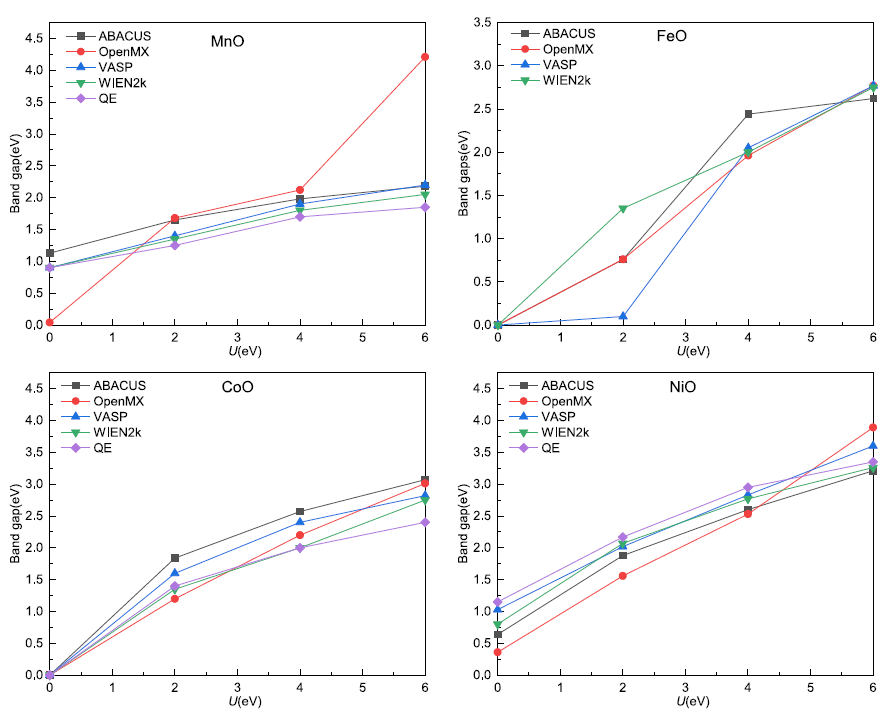
\includegraphics[width=0.75\textwidth]{figure/DFTU-diff-packages.png}\\
      \href{https://doi.org/10.1063/5.0090122}{\textcolor{blue}{\tiny{}J. Chem. Phys. 156, 234104 (2022)}}
    \end{figure}
  \end{frame}
  %-===================================================================-% 

  %+===================================================================+%
  \begin{frame}{Summary}
    \begin{block}{}
      \begin{itemize}
        \item The traditional DFT calculation method has two errors, (i) delocalization error (DE), and (ii) static correlated error (SCE). 
        
        \item The DE, which also called self-interaction error (SIE), is induced by the fact that density information alone cannot accurately describe the exchange term.
        
        \item In short, the DFT+\(U\) is to make a HF approximation to the Habburd model. It is simple, and efficient, but unrobust.
        
        \item The SCE is caused by the influence of quantum fluctuations with space and time. HF or DFT+\(U\) method cannot avoid it. Only the DMFT method can solve this kind of error.
      \end{itemize}
    \end{block}
  \end{frame}
  %-===================================================================-% 
\end{document} 